

\chapter{Readout Infidelity Budget}
With a simulation realistically representing the qubit-resonator system from the laboratory, we are now in a position to break down the different effects on the readout fidelity. In this section, we will leverage the simulation tools, to quantify the contributions to the infidelity from the different physical processes, we have included in our model. Thereafter, we will try to break down, how different improvements of the physical parameters will have an effect on the fidelity of our readout. 

\section{Estimating Contributions}

\begin{table}[h]
    \centering
    \begin{tabular}{l|r}
    \hline
         Parameters Set & Fidelity \\ \hline
         Realistic & 0.666  \\
         Perfect   & 0.985
    \end{tabular}

    \caption{Caption}
    \label{tab:my_label}
\end{table}


\begin{table}[h]
\centering
\caption{The outcome of calibrating the qubit with the methods presented in this chapter.}

\begin{tabular}{l|rrr}
\hline
\textbf{Contributions}        & Temperature     & Energy Decay   & Efficiency  \\ \hline
Excluding                     &  0.878          &  0.710         &  0.655 \\
Exclusively                   &  0.721          &  0.879         &  0.982
\end{tabular}
\label{tab:readout_infidelity_contribution_estimation}
\end{table}

\begin{figure*}
    \centering
    \missingfigure[figheight = \textheight / 3]{IQ Plots for the simulation, we ran in the table}
    \caption{Caption}
    \label{fig:enter-label}
\end{figure*}

There are many answers to which effect does what.

\section{Improving the Readout - Temperature}

\begin{figure}
    \centering
    \includegraphics{simulations/budgets/}
    \caption{Caption}
    \label{fig:enter-label}
\end{figure}

\begin{table}[h]
\centering
\caption{The outcome of calibrating the qubit with the methods presented in this chapter.}
\begin{tabular}{ll|r}
\hline
\textbf{Reduction}        & Temperature                  & Fidelity\\ \hline
-10 \%                     &  30                         &  99.99\\
0   \%                     &  30                         &  99.99\\
10  \%                     &  30                         &  99.99\\
25  \%                     &  30                         &  99.99\\
50  \%                     &  30                         &  99.99\\
100 \%                     &  30                         &  99.99\\
\end{tabular}
\label{tab:readout_infidelity_contribution_estimation}
\end{table}


\subsection{Active Reset}

\section{Improving the Readout - Qubit Decay}


\begin{table}[h]
\centering
\caption{The outcome of calibrating the qubit with the methods presented in this chapter.}
\begin{tabular}{ll|r}
\hline
\textbf{Reduction}        & Temperature                  & Fidelity\\ \hline
0   \%                      &  30                        &  99.99\\
10  \%                     &  30                         &  99.99\\
25  \%                     &  30                         &  99.99\\
50  \%                     &  30                         &  99.99\\
100 \%                     &  30                         &  99.99\\
\end{tabular}
\label{tab:readout_infidelity_contribution_estimation}
\end{table}



\subsection{Further Excitement}

\section{Improving the Readout - Efficiency}


\begin{table}[h]
\centering
\caption{The outcome of calibrating the qubit with the methods presented in this chapter.}
\begin{tabular}{ll|r}
\hline
\textbf{Reduction}        & Temperature                  & Fidelity\\ \hline
0   \%                      &  30                        &  99.99\\
10  \%                     &  30                         &  99.99\\
25  \%                     &  30                         &  99.99\\
50  \%                     &  30                         &  99.99\\
100 \%                     &  30                         &  99.99\\
\end{tabular}
\label{tab:readout_infidelity_contribution_estimation}
\end{table}



\subsection{High Power Readout}

\begin{figure}
    \centering
    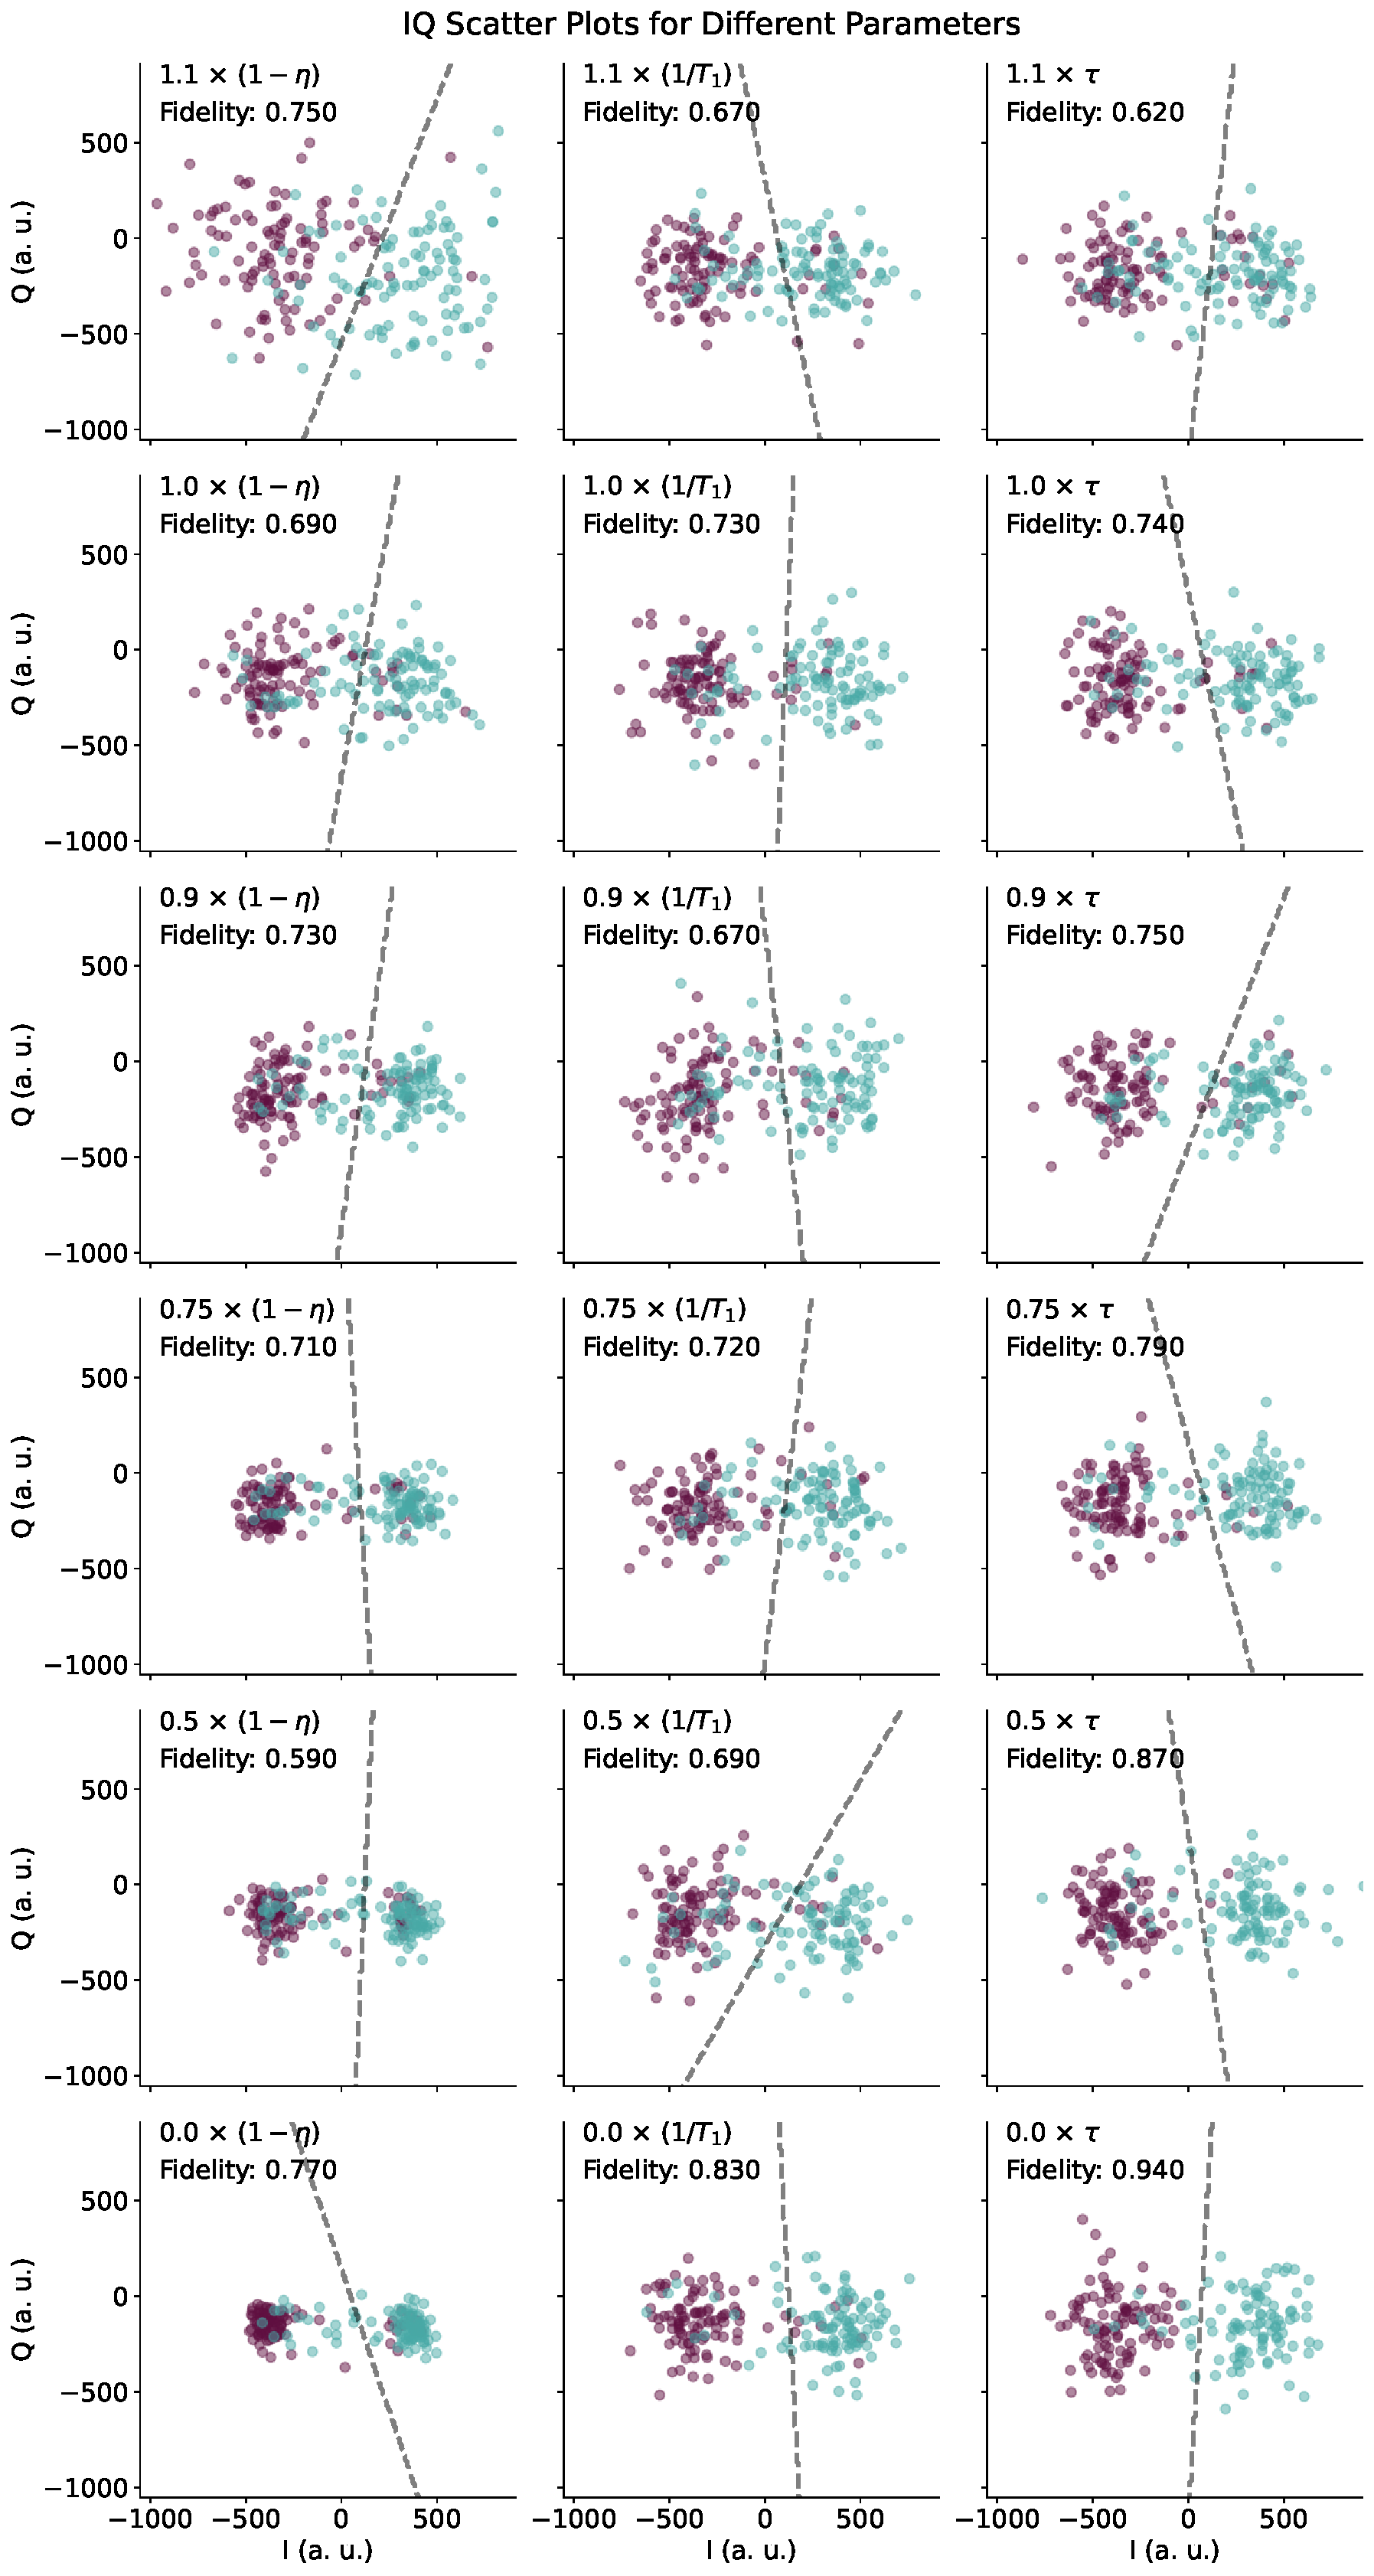
\includegraphics{Simulations/budgets/figures/iq_scatter_budgetting.pdf}
    \caption{The IQ Plots for the models  with different parameters. The seperation line, fidelity and parameter scaling is shown.}
    \label{fig:budgetting_IQ_plots}
\end{figure}


